\documentclass{beamer}
% imprimir
% \documentclass[handout]{beamer} 
% \usepackage{pgfpages}
% \pgfpagesuselayout{4 on 1}[a4paper,landscape,border shrink=5mm]

\mode<presentation> {
  \usetheme{Warsaw}
  \setbeamercovered{transparent}
}

\usebackgroundtemplate{\includegraphics[width=\paperwidth]{format/libresoft-bg.png}}
\usepackage[spanish]{babel}
\usepackage[utf8]{inputenc}
\usepackage{graphics}
\usepackage{amssymb} % Simbolos matematicos

%\definecolor{libresoftgreen}{RGB}{162,190,43}
%\definecolor{libresoftblue}{RGB}{0,98,143}

%\setbeamercolor{titlelike}{bg=libresoftgreen}

%% Metadatos del PDF.
\hypersetup{  
  pdftitle={Introducción a la administración de sistemas},
  pdfauthor={Miguel Vidal},
  pdfcreator={GSyC/Libresoft},
  pdfproducer=PDFLaTeX,
  pdfsubject={Introducción a la administración de sistemas},
}
%%

\begin{document}

\title{Introducción a la administración de sistemas}
\subtitle{Arquitectura de servidores con software libre}
\institute{\{mvidal,jfcastro\}@gsyc.urjc.es} 
\author{Miguel Vidal, Jos\'{e} Castro}
%\date{\today}
\date{25 de marzo de 2011}

\frame{
\maketitle
\begin{center}

\includegraphics[width=6cm]{format/gsyc-urjc}
\end{center}
}

\frame{
~
\vspace{4cm}

\begin{flushright}
{\small
(cc) 2009-2011 Miguel Vidal, José Castro. \\
  Esta presentación se publica bajo una licencia Creative Commons Reconocimiento 3.0 España, disponible en 
  \url{http://creativecommons.org/licenses/by/3.0/es/}
 

\bigskip

}
\end{flushright}
}
%%

\begin{frame}
  \frametitle{Agenda}

%  \begin{itemize}[<+->]
\begin{enumerate}
\item ¿Qué es un administrador de sistemas? 
\item Tipos de sysadmin
\item Deberes de un sysadmin. Cultura (\textsc{bofh}, Usenet\dots)
\item Políticas y procedimientos
\item Sistemas de seguimiento de incidencias
\item Constelación de los sistemas operativos libres de Unix
\item Asociaciones y organizaciones profesionales, certificaciones     
\end{enumerate}

\end{frame}

%%%%%%%%%%%%%%%%%%%%%%%%%%%%%%%%%%%%%%%%%%%%%%%%%%%%%%%%%%%%%%%%%%%%%%%
\section{¿Qué es un administrador de sistemas?}
%%%%%%%%%%%%%%%%%%%%%%%%%%%%%%%%%%%%%%%%%%%%%%%%%%%%%%%%%%%%%%%%%%%%%%%

\begin{frame}

\begin{center}
\huge{¿Qué es un administrador de sistemas?}
\end{center}

\end{frame}


%%%%%%%%%%%%%%%%%%%%%%%%%%%%%%%%%%%%%%%%%%%%%%%%%%%%%%%%%%%%%%%%%%%%%%%

\begin{frame}
\frametitle{¿Qué es un administrador de sistemas?}

``\textit{Un administrador de sistemas es aquel profesional que tiene la responsabilidad de ejecutar, mantener, operar y asegurar el correcto funcionamiento de un sistema informático y/o una red de ordenadores.}'' (Wikipedia).

\bigskip

Tambien llamado \alert{sysadmin}, debe demostrar una mezcla de \alert{cualidades técnicas} y de \alert{responsabilidad} para desempeñar bien su trabajo. 

\end{frame}

%%%%%%%%%%%%%%%%%%%%%%%%%%%%%%%%%%%%%%%%%%%%%%%%%%%%%%%%%%%%%%%%%%%%%%%

\begin{frame}
\frametitle{Tareas esenciales de la administración de sistemas}

\begin{itemize}
\item Istalación, soporte y mantenimiento de servidores o de otros sistemas informáticos.
\item \textit{Scripting} o programación ligera. 
\item Gestión de proyectos en proyectos relacionados con sistemas. 
\item Supervisión y formación de operadores. 
\item mantenimiento: Monitorización del sistema, ejecutar backups, actualizar software, añadir y retirar hardware...
\item Creación, organización y mantenimiento de la documentación.
\item Soporte a usuarios.
\end{itemize}

\small

Todas estas tareas no necesariamente las lleva a cabo una sola persona. Pero al menos una persona debe conocerlas y asegurarse de que alguien las hace.

\end{frame}


%%%%%%%%%%%%%%%%%%%%%%%%%%%%%%%%%%%%%%%%%%%%%%%%%%%%%%%%%%%%%%%%%%%%%%%

\begin{frame}
\frametitle{Habilidades, formación}

\begin{itemize}
\item La administración de sistemas implica más cambios de contextos en un solo día que la mayoría de trabajos en un año.

\item Un sysadmin necesita habilidad para organizarse y gestionar su tiempo eficientemente.
\item Habilidad para mantener felices a los usuarios en una situación \textit{win-win}.
\item El ``queme'' en el trabajo de un sysadmins es creciente. La mayoría de los administradores duran solo unos cuantos años.
\item A diferencia de otras profesiones, no existe una única vía para convertirse en sysadmin.
\end{itemize}
\end{frame}

%%%%%%%%%%%%%%%%%%%%%%%%%%%%%%%%%%%%%%%%%%%%%%%%%%%%%%%%%%%%%%%%%%%%%%%

\begin{frame}
\frametitle{Habilidades}

\begin{itemize}
\item Tenacidad para resolver problemas (incluso obsesivos).
\item Deseo genuino de ayudar a la gente.
\item Los sysadmins suelen considerar divertido lo que hacen.
\end{itemize}
\end{frame}


%%%%%%%%%%%%%%%%%%%%%%%%%%%%%%%%%%%%%%%%%%%%%%%%%%%%%%%%%%%%%%%%%%%%%%%
\section{Tipos de sysadmin}
%%%%%%%%%%%%%%%%%%%%%%%%%%%%%%%%%%%%%%%%%%%%%%%%%%%%%%%%%%%%%%%%%%%%%%%


\begin{frame}
\frametitle{Tipos de sysadmin}

\begin{itemize}
\item senior
\item operador
\item soporte técnico 
\item administrador de base de datos (DBA)
\item administrador de seguridad
\item administrador web
\end{itemize}
\end{frame}



%%%%%%%%%%%%%%%%%%%%%%%%%%%%%%%%%%%%%%%%%%%%%%%%%%%%%%%%%%%%%%%%%%%%%%%
% \section{Duties of a system administrator}
%%%%%%%%%%%%%%%%%%%%%%%%%%%%%%%%%%%%%%%%%%%%%%%%%%%%%%%%%%%%%%%%%%%%%%%




%%%%%%%%%%%%%%%%%%%%%%%%%%%%%%%%%%%%%%%%%%%%%%%%%%%%%%%%%%%%%%%%%%%%%%%
\section{Políticas y procedimientos}
%%%%%%%%%%%%%%%%%%%%%%%%%%%%%%%%%%%%%%%%%%%%%%%%%%%%%%%%%%%%%%%%%%%%%%%


\begin{frame}

\begin{center}
\huge{Políticas y procedimientos}
\end{center}

\end{frame}

%%%%%%%%%%%%%%%%%%%%%%%%%%%%%%%%%%%%%%%%%%%%%%%%%%%%%%%%%%%%%%%%%%%%%%%

\begin{frame}
\frametitle{Documentación}

\begin{itemize}
\item Páginas \texttt{man}: tradicional doc. online.
	\begin{itemize}
	\item Están organizadas por secciones. 
	\item Una misma orden puede estar en varias secciones.
	\item No son howtos. 
\item GNU Texinfo (Linux)
\item Guías y documentación específica de cada sistema (ej. \textit{FreeBSD Handbook} o \texttt{docs.sun.com})
\item Documentación específica del paquete: (ej. \texttt{/usr/share/doc})
\item Libros en papel (O'Reilly)
\item Linux Documentation Project
\item RFCs
\end{itemize}

\end{frame}


%%%%%%%%%%%%%%%%%%%%%%%%%%%%%%%%%%%%%%%%%%%%%%%%%%%%%%%%%%%%%%%%%%%%%%%

\begin{frame}
\frametitle{Importancia de documentar}

\begin{itemize}
\item La documentación ayuda a la reproducibilidad. 
\item La documentación ahorra tiempo. 
\item La documentación reduce la propabilidad de puntos únicos de fallo (SPoF).
\item Lo principal: la documentación mejora la inteligibilidad de un sistema y permite que
	las modificaciones se hagan de un modo consistente.
\item Escribe documentos cortos: de una página que cubran un solo tema.
\item La documentación local debe guardarse en un solo punto bien definido (wiki, repo...).
\end{itemize}

\end{frame}


%%%%%%%%%%%%%%%%%%%%%%%%%%%%%%%%%%%%%%%%%%%%%%%%%%%%%%%%%%%%%%%%%%%%%%%


%%%%%%%%%%%%%%%%%%%%%%%%%%%%%%%%%%%%%%%%%%%%%%%%%%%%%%%%%%%%%%%%%%%%%%%

\begin{frame}
\frametitle{Procedimientos}

Algunas tareas comunes que suelen necesitar procedimientos:

\begin{itemize}
\item Adding a host
\item Adding a user
\item Setting up backups for a new machine
\item Securing a new machine
\item Upgrading the operating system
\item Backing up and restoring files
\item Performing emergency shutdowns
\item Handling of security break-ins
\end{itemize}
\end{frame}

%%%%%%%%%%%%%%%%%%%%%%%%%%%%%%%%%%%%%%%%%%%%%%%%%%%%%%%%%%%%%%%%%%%%%%%

\begin{frame}
\frametitle{Políticas}

Políticas habituales:

\begin{itemize}
\item Políticas de seguridad
\item Políticas para los administradores (login, sudo, pfexec...)
\item Acceso y políticas de usuario
\item Política de privacidad
\item Cuestiones legales: copyright (licencias y datos almacenados), cifrado, protección de datos personales...
\end{itemize}
\end{frame}


%%%%%%%%%%%%%%%%%%%%%%%%%%%%%%%%%%%%%%%%%%%%%%%%%%%%%%%%%%%%%%%%%%%%%%%
\section{Issue tracking system and trouble-reporting system}
%%%%%%%%%%%%%%%%%%%%%%%%%%%%%%%%%%%%%%%%%%%%%%%%%%%%%%%%%%%%%%%%%%%%%%%


\begin{frame}
\frametitle{What is an issue tracking system}

\begin{itemize}
\item Software to create, update, and resolve reported lists of issues. Similar to a "bugtracker".
\item Contains a knowledge base with resolutions to common problems: invaluable resource for the sysadmin staff.
\item Ticket/Issue: a file which contains information about support interventions made by technical support staff.
\item Trac (python), RT (Perl), Redmine (RoR), OTRS, Mantis...: \url{http://en.wikipedia.org/wiki/Comparison_of_issue_tracking_systems}

\end{itemize}
\end{frame}

%%%%%%%%%%%%%%%%%%%%%%%%%%%%%%%%%%%%%%%%%%%%%%%%%%%%%%%%%%%%%%%%%%%%%%%


\begin{frame}
\frametitle{Common functions of trouble ticket systems}

Managers can extract high-level information such as:
\begin{itemize}
\item The number of open tickets
\item The average time to close a ticket
\item The productivity of sysadmins
\item The percentage of unresolved tickets
\item Workload distribution by time to solution

\end{itemize}
\end{frame}


%%%%%%%%%%%%%%%%%%%%%%%%%%%%%%%%%%%%%%%%%%%%%%%%%%%%%%%%%%%%%%%%%%%%%%%

\begin{frame}
\frametitle{Workflow}

\begin{itemize}
\item User (or helpdesk) reports a problem.
\item Operator verifies that the problem is real, and not just perceived. 
\item Operator will also ensure that enough information about the problem is obtained from the user.
\item After the issue has been fully addressed, it is marked as resolved/closed/wontfix/feedback...

\end{itemize}
\end{frame}

%%%%%%%%%%%%%%%%%%%%%%%%%%%%%%%%%%%%%%%%%%%%%%%%%%%%%%%%%%%%%%%%%%%%%%%

\begin{frame}
\frametitle{Redmine}

Main features:
\begin{itemize}
\item Multiple projects support
\item ACL's: Flexible role-based access control
\item Per project wiki 
\item SCM integration (SVN, CVS, Git, Mercurial, Bazaar and Darcs)
\item User self-registration support
\item Gantt chart and calendar
\item Feeds \& e-mail notifications.
\end{itemize}
\end{frame}


%%%%%%%%%%%%%%%%%%%%%%%%%%%%%%%%%%%%%%%%%%%%%%%%%%%%%%%%%%%%%%%%%%%%%%%
\section{Free/Open Unix-like constellation}
%%%%%%%%%%%%%%%%%%%%%%%%%%%%%%%%%%%%%%%%%%%%%%%%%%%%%%%%%%%%%%%%%%%%%%%

\begin{frame}
\frametitle{Certificación UNIX}

\begin{itemize}
\item \textsc{UNIX}\texttrademark{} es una marca registrada propiedad del Open Group consortium (Fujitsu, Sun, Hitachi, HP, IBM, NEC, US DoD, la NASA y otros). 
\item Open Group se encarga de conceder certificados SUS: Single UNIX Specification 
\item Solaris, HP-UX, AIX y MacOS X tienen certificación SUS
\item Tipo Unix (\textit{Unix-like}): Linux, BSD y OpenSolaris
\end{itemize}
\end{frame}


%%%%%%%%%%%%%%%%%%%%%%%%%%%%%%%%%%%%%%%%%%%%%%%%%%%%%%%%%%%%%%%%%%%%%%%

\begin{frame}
\frametitle{A brief history about Unix and SunOS/Solaris}
\begin{center}
  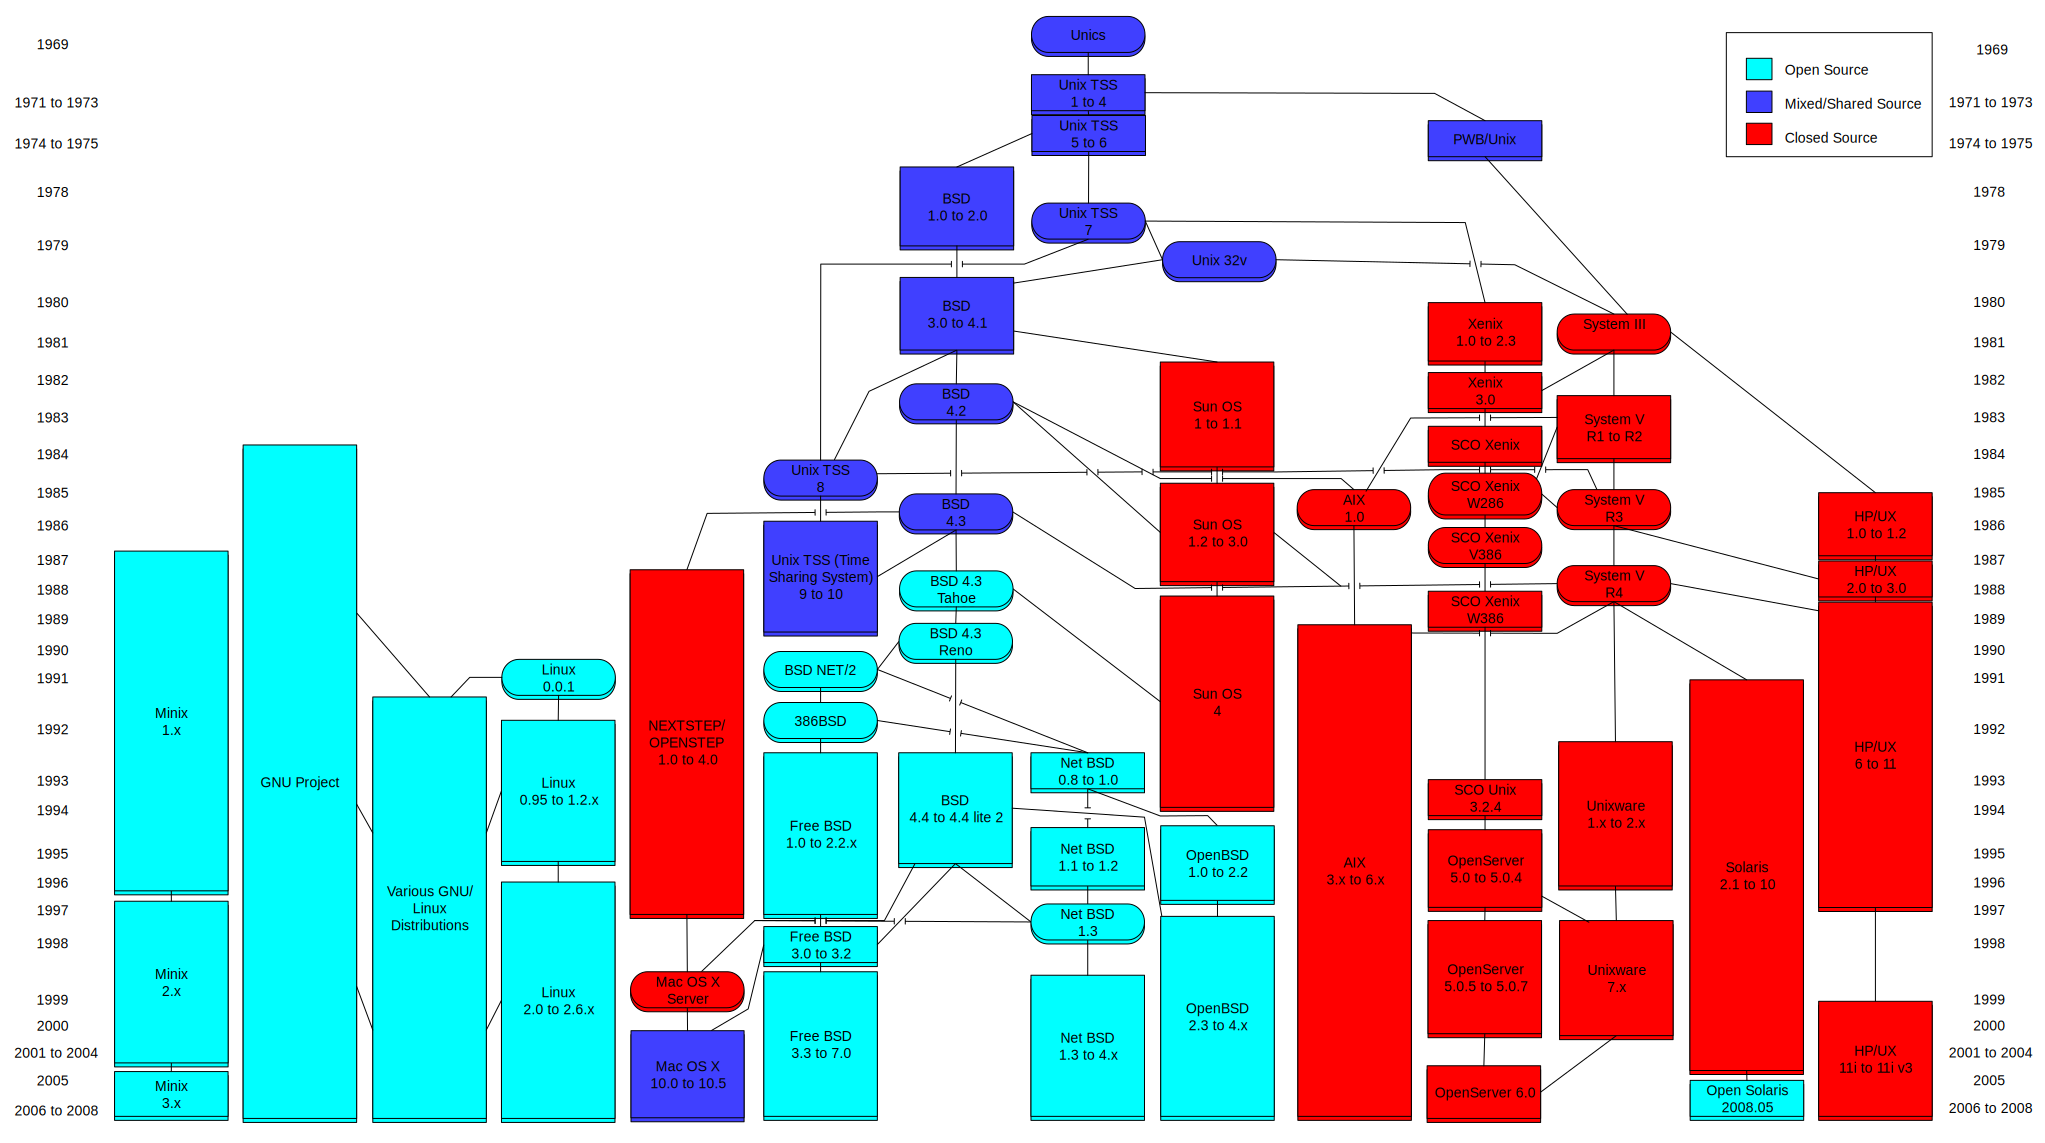
\includegraphics[height=2.5in]{figs/Unix_history-simple.png}
\end{center}
\end{frame}

%%%%%%%%%%%%%%%%%%%%%%%%%%%%%%%%%%%%%%%%%%%%%%%%%%%%%%%%%%%%%%%%%%%%%%%

\begin{frame}
\frametitle{A brief history about Unix and SunOS/Solaris}
\begin{center}
  \includegraphics[height=2.7in]{figs/Unix_history.png}
\end{center}
\end{frame}

%%%%%%%%%%%%%%%%%%%%%%%%%%%%%%%%%%%%%%%%%%%%%%%%%%%%%%%%%%%%%%%%%%%%%%%

\begin{frame}
\frametitle{Linux and Unix}

\begin{itemize}
\item Linux is a reimplementation and elaboration of UNIX. 
\item It conforms to the POSIX standard, runs on several hardware platforms, and is compatible with most existing UNIX software.
\item Linux incorporates technical refinements that did not exist in the original versions of UNIX, so it is more than just a UNIX clone.
\item It is also a legally distinct entity and cannot be properly be referred to as ``UNIX''
\item From the standpoint of applications, Linux software is UNIX software (thanks to GNU Project). 
\end{itemize}
\end{frame}

%%%%%%%%%%%%%%%%%%%%%%%%%%%%%%%%%%%%%%%%%%%%%%%%%%%%%%%%%%%%%%%%%%%%%%%

\begin{frame}
\frametitle{Another free Unix-like systems}

\begin{itemize}
\item FreeBSD, NetBSD, and OpenBSD, from UC Berkeley. 
\item It conforms to the POSIX standard, runs on several hardware platforms, and is compatible with most existing UNIX software.
\item These OSes are comparable to Linux in features and reliability, although they enjoy somewhat less support from third-party software vendors.
\end{itemize}
\end{frame}

%%%%%%%%%%%%%%%%%%%%%%%%%%%%%%%%%%%%%%%%%%%%%%%%%%%%%%%%%%%%%%%%%%%%%%%

\begin{frame}
\frametitle{Free Unix systems: OpenSolaris}

\begin{itemize}
\item A new FLOSS operating system based on source code of Solaris. 
\item The bulk of the Solaris system code was released on June 14, 2005
\item The only libre software SVR4 derivative available.
\item An attempt to use a community development model to develop Solaris.
\item Supported by Sun/Oracle. Future commercial versions of Solaris will based around OpenSolaris code!
\item Unique features: ZFS, zones, crossbow...
\end{itemize}
\end{frame}

%%%%%%%%%%%%%%%%%%%%%%%%%%%%%%%%%%%%%%%%%%%%%%%%%%%%%%%%%%%%%%%%%%%%%%%
\section{Associations and professional organizations}
%%%%%%%%%%%%%%%%%%%%%%%%%%%%%%%%%%%%%%%%%%%%%%%%%%%%%%%%%%%%%%%%%%%%%%%

\begin{frame}

\begin{center}
\huge{Asociaciones y organizaciones profesionales}
\end{center}

\end{frame}

%%%%%%%%%%%%%%%%%%%%%%%%%%%%%%%%%%%%%%%%%%%%%%%%%%%%%%%%%%%%%%%%%%%%%%%

\begin{frame}
\frametitle{SAGE}

\begin{itemize}
\item Es la primera organización internacional para sysadmins.
\item Es un grupo de interés dentro de Usenix.
\item Promueve la admnistración de sistemas como profesión y patrocina confenrencias y programas informales.
\item Organiza el mayor evento para sysadmins: la conferencia USENIX LISA (Large Installation System Administration) en otoño.
\item SAGE se enfoca más a la investigación.
\end{itemize}
\end{frame}

%%%%%%%%%%%%%%%%%%%%%%%%%%%%%%%%%%%%%%%%%%%%%%%%%%%%%%%%%%%%%%%%%%%%%%%


\begin{frame}
\frametitle{LOPSA}

\begin{itemize}
\item LOPSA, the League of Professional System Administrators.
\item In 2005, some of the old-timers in the SAGE organization formed a separate organization called LOPSA
\item Mission: to advance the practice of system administration; to support, recognize, educate, and encourage its practitioners; and to serve the public through education and outreach on system administration issues.
\item LOPSA seeks to provide legislative advocacy and to help mold legislative policy on issues effecting the profession. 
\item SAGE and LOPSA cooperate on common goals such as the Code of Ethics and the LISA conference.
\end{itemize}
\end{frame}

%%%%%%%%%%%%%%%%%%%%%%%%%%%%%%%%%%%%%%%%%%%%%%%%%%%%%%%%%%%%%%%%%%%%%%%

\begin{frame}
\frametitle{Unix Culture}

\begin{itemize}
\item ``KISS'', ``Small is beautiful'', ``Make each program do one thing well'', ``Build a prototype as soon as possible'', ``Choose portability over efficiency'', ``Use shell scripts to increase leverage and portability'', ``Avoid captive user interfaces'', ``Make every program a filter''...
\item ``Worse is better'': design style and simplicity is more important than correctness, consistency and completeness.
\item Usenet, Internet jargon... 
\item System Administrator Appreciation Day (last Friday in July)
\item Bastard Operator From Hell (BOFH)
\end{itemize}
\end{frame}


%%%%%%%%%%%%%%%%%%%%%%%%%%%%%%%%%%%%%%%%%%%%%%%%%%%%%%%%%%%%%%%%%%%%%%%

\begin{frame}
\frametitle{Código ético (1)}

LOPSA, USENIX, y SAGE animan a que todo administrador se guía por un código ético:  

\begin{itemize}
\item Profesionalidad
\item Integridad personal
\item Privacidad
\item Leyes y políticas
\item Communicación
\end{itemize}
\end{frame}

%%%%%%%%%%%%%%%%%%%%%%%%%%%%%%%%%%%%%%%%%%%%%%%%%%%%%%%%%%%%%%%%%%%%%%%

\begin{frame}
\frametitle{Código ético (2)}

\begin{itemize}
\item Integridad de sistema
\item Educación
\item Responsibilidad social
\item Responsibilidad ética
\end{itemize}

\url{http://lopsa.org/CodeOfEthics}

\end{frame}

%%%%%%%%%%%%%%%%%%%%%%%%%%%%%%%%%%%%%%%%%%%%%%%%%%%%%%%%%%%%%%%%%%%%%%%

\begin{frame}
\frametitle{Referencias}

\begin{itemize}
\item Nemeth, Snyder, Hein \textit{UNIX and Linux System Administration Handbook}
\item Limoncelli, Thomas A. \textit{Time Management for System Administrators} 
\end{itemize}

\end{frame}


\end{document}




